\thispagestyle{empty}
\chapter{Mapping for Autonomous Vehicles}  
\thispagestyle{empty}  
\label{cpt:mapping}  

This chapter introduces readers to the complete technology stack for point cloud mapping and high-definition (HD) maps in autonomous driving. Full point cloud mapping can be viewed as a comprehensive optimization problem involving RTK, IMU, wheel odometry, and LiDAR. Most L4-level autonomous driving tasks require a complete, RTK-aligned point cloud map for tasks such as map annotation and high-precision localization. We will progressively cover the entire process of point cloud mapping: frontend, backend, loop closure detection, map segmentation, and export. These steps are largely similar across most applications.  

In this chapter, we will work with readers to implement a complete point cloud mapping system, where some components can be straightforwardly assembled using algorithmic modules from previous chapters. This system can start from offline data packets, construct, and export point cloud maps that are practically usable for high-precision localization. We will also briefly introduce some vector map-related content. However, since the annotation and generation of vector HD maps are not closely related to SLAM algorithms, we will not require readers to perform map annotation tasks themselves. The next chapter of this book will also use the point cloud maps constructed in this chapter for actual fusion-based localization algorithm testing.  

\includepdf[width=\textwidth]{art/ch9.pdf}

\section{Point Cloud Mapping Pipeline}  
Unlike online SLAM systems, mapping systems can operate entirely in offline mode. A major advantage of offline systems is their strong determinism. Each algorithmic step—how it should be executed and what output it should produce—can be planned and determined in advance. There are no scheduling issues related to threads or resources between modules, whereas online systems often need to consider inter-thread dependencies, such as whether to insert new submaps before loop closure detection completes or whether to allow exporting maps with unclosed loops. Therefore, designing a mapping framework as an offline system is easier than developing a real-time SLAM system and enables better automation capabilities.  

\begin{figure}  
	\centering  
	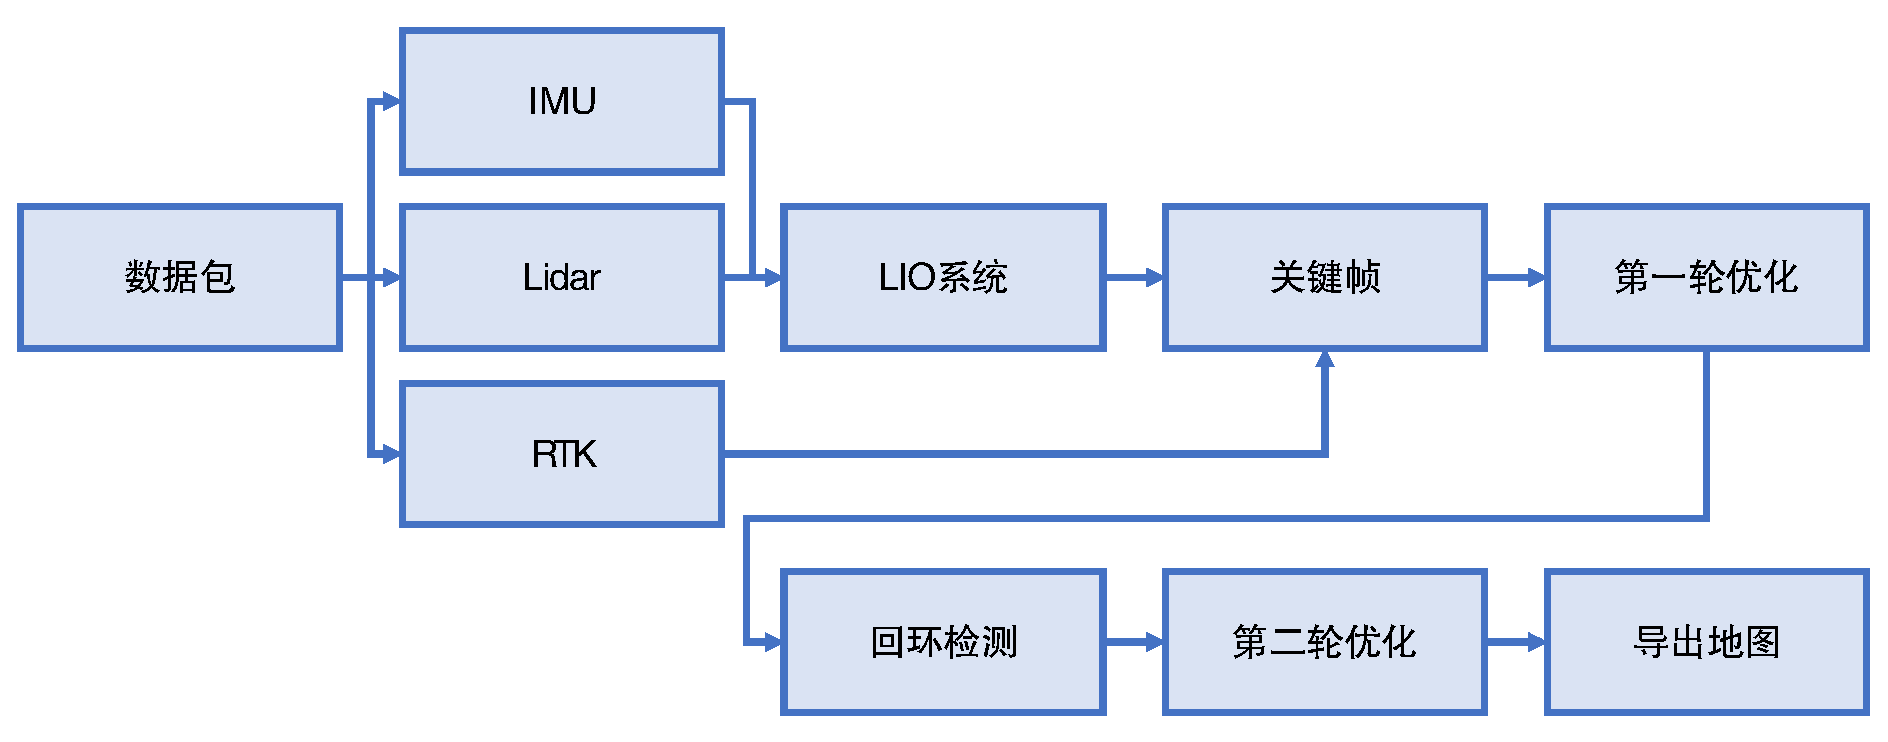
\includegraphics[width=0.8\textwidth]{mapping/mapping-pipeline.pdf}  
	\caption{The workflow framework of the mapping system}  
	\label{fig:mapping-pipeline}  
\end{figure}  

We design the entire mapping pipeline following the approach in \cite{Gao2021}, as shown in Fig.~\ref{fig:mapping-pipeline}.  

\begin{enumerate}  
	\item First, we extract IMU, RTK, and LiDAR data from the given ROS bag. Due to dataset variability, not all datasets include wheel odometry (and wheel odometry formats often vary by vehicle). Thus, we primarily use IMU and LiDAR data to construct the LIO system. This part directly utilizes the IEKF LIO code from the previous chapter.  
	\item Most autonomous vehicles are also equipped with RTK devices or integrated navigation systems. These devices provide the vehicle's position in the physical world but may suffer from signal interference. In the LIO system, we collect point cloud keyframes at certain intervals and assign each keyframe an RTK pose (as an observation) based on RTK or integrated navigation data. This book primarily uses the NCLT dataset (Fig.~\ref{fig:nclt-car}) as an example, where the RTK signal follows a single-antenna solution, providing only positional data without orientation.  
	\item Next, we use LIO for inter-frame motion estimation and RTK poses as absolute coordinate observations to optimize the entire trajectory and determine the validity of RTK for each keyframe. This is called the **first-round optimization**. If RTK functions normally, we obtain a trajectory roughly aligned with RTK. However, in real-world environments, RTK often has invalid observations, which must be identified in the algorithm.  
	\item Based on the previous step, we perform loop closure detection on the map. The detection algorithm can simply use Euclidean distance-based checks, with NDT or common registration algorithms computing their relative poses. This example employs multi-resolution NDT matching for loop closure detection.  
	\item Finally, we integrate all this information into a unified pose graph for optimization, eliminating ghosting caused by accumulated errors and removing regions where RTK fails. This is called the **second-round optimization**. Once the poses are finalized, we export the point cloud map accordingly. For easier map loading and visualization, we also segment the point cloud map into tiles. The processed point cloud can then be used for high-precision localization or map annotation.  
\end{enumerate}  

\begin{figure}  
	\centering  
	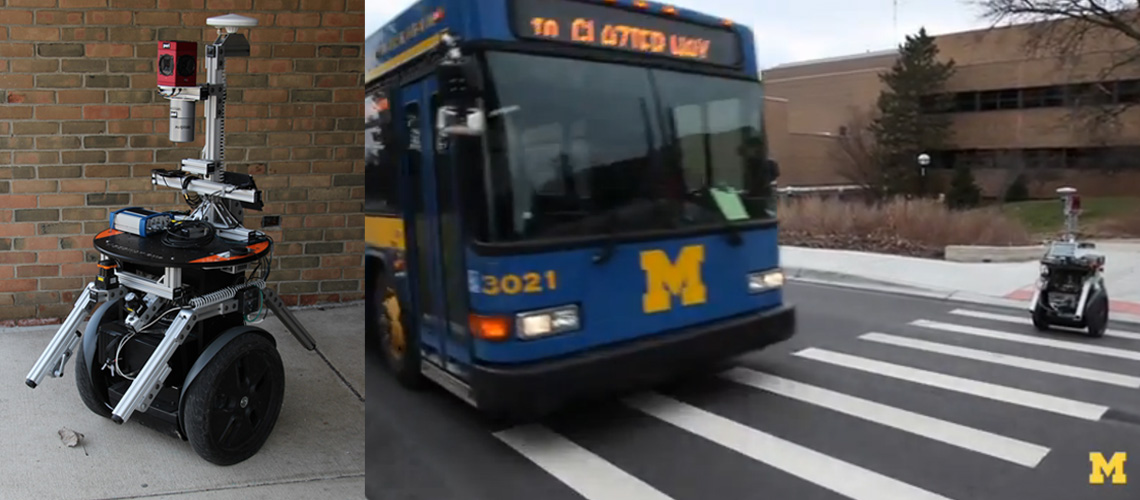
\includegraphics[width=0.8\textwidth]{mapping/NCLT-car.jpg}  
	\caption{The vehicle used in the NCLT dataset, image from \cite{CarlevarisBianco2015}}  
	\label{fig:nclt-car}  
\end{figure}

\section{Frontend Implementation}
First, we implement the frontend. Since previous chapters have already covered a complete LIO system, we only need to add some peripheral logic for data packet parsing. The main frontend code is located in:

\begin{lstlisting}[language=c++,caption=src/ch9/frontend.cc]
void Frontend::Run() {
	sad::RosbagIO rosbag_io(bag_path_, DatasetType::NCLT);
	
	// First extract RTK poses (note NCLT only has translation components)
	rosbag_io
	.AddAutoRTKHandle([this](GNSSPtr gnss) {
		gnss_.emplace(gnss->unix_time_, gnss);
		return true;
	})
	.Go();
	rosbag_io.CleanProcessFunc();  // No longer need to process RTK
	
	RemoveMapOrigin();
	
	// Then run LIO
	rosbag_io
	.AddAutoPointCloudHandle([&](sensor_msgs::PointCloud2::Ptr cloud) -> bool {
		lio_->PCLCallBack(cloud);
		ExtractKeyFrame(lio_->GetCurrentState());
		return true;
	})
	.AddImuHandle([&](IMUPtr imu) {
		lio_->IMUCallBack(imu);
		return true;
	})
	.Go();
	lio_->Finish();
	
	// Save running results
	SaveKeyframes();
	
	LOG(INFO) << "done.";
}
\end{lstlisting}

As can be seen, the frontend mainly performs the following tasks:
\begin{enumerate}
	\item Extracts RTK data from the ROS bag and stores it in an RTK message queue, sorted by acquisition time.
	\item Uses the first valid RTK data as the map origin, then subtracts this origin from other RTK readings to use them as RTK position observations.
	\item Runs LIO using IMU and LiDAR data, extracts keyframes based on distance and angle thresholds, and finally saves the keyframe results.
\end{enumerate}

\section{Keyframe Extraction}
When extracting keyframes, we also retrieve their poses and point clouds from the LIO system:
\begin{lstlisting}[language=c++,caption=src/ch9/frontend.cc]
void Frontend::ExtractKeyFrame(const sad::NavStated& state) {
	if (last_kf_ == nullptr) {
		// First frame
		auto kf = std::make_shared<Keyframe>(state.timestamp_, kf_id_++, state.GetSE3(), lio_->GetCurrentScan());
		FindGPSPose(kf);
		kf->SaveAndUnloadScan("./data/ch9/");
		keyframes_.emplace(kf->id_, kf);
		last_kf_ = kf;
	} else {
		// Calculate motion thresholds between current state and last keyframe
		SE3 delta = last_kf_->lidar_pose_.inverse() * state.GetSE3();
		if (delta.translation().norm() > kf_dis_th_ || delta.so3().log().norm() > kf_ang_th_deg_ * math::kDEG2RAD) {
			auto kf = std::make_shared<Keyframe>(state.timestamp_, kf_id_++, state.GetSE3(), lio_->GetCurrentScan());
			FindGPSPose(kf);
			keyframes_.emplace(kf->id_, kf);
			kf->SaveAndUnloadScan("./data/ch9/");
			LOG(INFO) << "Generated keyframe" << kf->id_;
			last_kf_ = kf;
		}
	}
}
\end{lstlisting}

These point clouds are sequentially stored in the data/ch9/ directory and then cleared from memory. Meanwhile, we query the RTK pose queue by timestamp, calling a generic pose interpolation function from the math library:

\begin{lstlisting}[language=c++,caption=src/ch9/frontend.cc]
void Frontend::FindGPSPose(std::shared_ptr<Keyframe> kf) {
	SE3 pose;
	GNSSPtr match;
	if (math::PoseInterp<GNSSPtr>(
	kf->timestamp_, gnss_, [](const GNSSPtr& gnss) -> SE3 { return gnss->utm_pose_; }, pose, match)) {
		kf->rtk_pose_ = pose;
		kf->rtk_valid_ = true;
	} else {
		kf->rtk_valid_ = false;
	}
}

/**
* Pose interpolation algorithm
* @tparam T    Data type
* @param query_time Query time
* @param data  Data container
* @param take_pose_func Pose extraction predicate
* @param result Interpolation result
* @param best_match_iter Closest matched element
*
* NOTE: query_time must be within data's time range (no extrapolation)
* Data map must be time-sorted
* @return Whether interpolation succeeded
*/
template <typename T>
bool PoseInterp(double query_time, const std::map<double, T>& data, const std::function<SE3(const T&)>& take_pose_func,
SE3& result, T& best_match) {
	if (data.empty()) {
		LOG(INFO) << "data is empty";
		return false;
	}
	
	if (query_time > data.rbegin()->first) {
		LOG(INFO) << "query time is later than last, " << std::setprecision(18) << ", query: " << query_time
		<< ", end time: " << data.rbegin()->first;
		
		return false;
	}
	
	auto match_iter = data.begin();
	for (auto iter = data.begin(); iter != data.end(); ++iter) {
		auto next_iter = iter;
		next_iter++;
		
		if (iter->first < query_time && next_iter->first >= query_time) {
			match_iter = iter;
			break;
		}
	}
	
	auto match_iter_n = match_iter;
	match_iter_n++;
	assert(match_iter_n != data.end());
	
	double dt = match_iter_n->first - match_iter->first;
	double s = (query_time - match_iter->first) / dt;  // s=0: first frame, s=1: next frame
	
	SE3 pose_first = take_pose_func(match_iter->second);
	SE3 pose_next = take_pose_func(match_iter_n->second);
	result = {pose_first.unit_quaternion().slerp(s, pose_next.unit_quaternion()),
		pose_first.translation() * (1 - s) + pose_next.translation() * s};
	best_match = s < 0.5 ? match_iter->second : match_iter_n->second;
	return true;
}
\end{lstlisting}

This function can retrieve poses from any map structure (requiring user-provided pose extraction method) and perform interpolation. For RTK readings, we simply return its utm_pose. Thus, we obtain the corresponding LIO pose, RTK pose, and scanned point cloud for each keyframe. All this data is stored in the data/ch9/ directory for subsequent algorithm modules.

Now please compile and run the frontend test program:
\begin{lstlisting}[language=sh,caption=Terminal command:]
bin/run_frontend --config_yaml ./config/mapping.yaml
\end{lstlisting}

This program reads basic information like data directory from the YAML configuration file and runs the entire frontend. The computation may take some time. Upon completion, you should see a series of PCD files and a keyframes.txt pose data file in ./data/ch9/, with content similar to:

\begin{lstlisting}[language=sh,caption=keyframes.txt]
0 1326652772.63223195 0 1 1 0.00323679756335721767 -0.0144500186628650669 0.00648581949310997503 0.00102604343126653629 -0.000610794694837971455 -0.00292974916442335183 0.999994995354752558 0 0 0 0 0 0 1 0 0 0 0 0 0 1 0 0 0 0 0 0 1 
1 1326652810.69380093 0 1 1 -0.00878834742957286877 0.00258137652733943018 -0.0370536530158143834 0.00556325961406906912 -0.000227692342581170451 0.0937748334061895006 0.995577861806049347 -0.00207286058563104208 0.00403151070086457675 0.00941915643412104611 0 0 0 1 0 0 0 0 0 0 1 0 0 0 0 0 0 1 
2 1326652811.20330048 0 1 1 0.00422691408508832616 -0.0517418751056824486 -0.0160935510000861509 0.0231508342749745313 -0.00193957036575541104 0.191042271176856737 0.981306846792967979 -0.00323174750160585156 0.0129979040447824497 0.0161721026594033174 0 0 0 1 0 0 0 0 0 0 1 0 0 0 0 0 0 1 
3 1326652813.51224709 0 1 1 0.401907347299137463 -0.959786854845477433 -0.0772027821235120038 0.108749752190681712 0.0143241272304329356 0.187688702845765748 0.976084659034054059 -0.0201519057154655457 0.305439419113099575 0.0159999999999627107 0 0 0 1 0 0 0 0 0 0 1 0 0 0 0 0 0 1 
4 1326652814.32679105 0 1 1 0.764588972100686437 -1.91970590325136792 -0.0977756250833726193 0.0454533237407165613 -0.0122335876446319734 0.187788495604154393 0.981080942436958869 -0.268586141930427402 0.693511614575982205 0.0269999999999868123 0 0 0 1 0 0 0 0 0 0 1 0 0 0 0 0 0 1 
\end{lstlisting}

This file records various poses (RTK, LiDAR odometry, backend-optimized) for each keyframe. Currently only RTK and LiDAR odometry poses are valid since we've only run the frontend. Later we'll use this information for loop closure detection and pose optimization. Now you can merge these keyframe point clouds into a complete map using the frontend-estimated poses:
\begin{lstlisting}[language=sh,caption=Terminal command:]
bin/dump_map --pose_source=lidar
\end{lstlisting}

Readers can examine dump_map.cc to see how map merging works. This command generates a map.pcd file in ./data/ch9/, which can be viewed using pcl_viewer as shown in Fig~\ref{fig:nclt-frontend}. The frontend structure appears locally accurate but inevitably exhibits accumulated errors, with noticeable ghosting in repeatedly visited areas. Don't worry - subsequent fusion optimization and loop closure detection will naturally eliminate these artifacts.

\begin{figure}
	\centering
	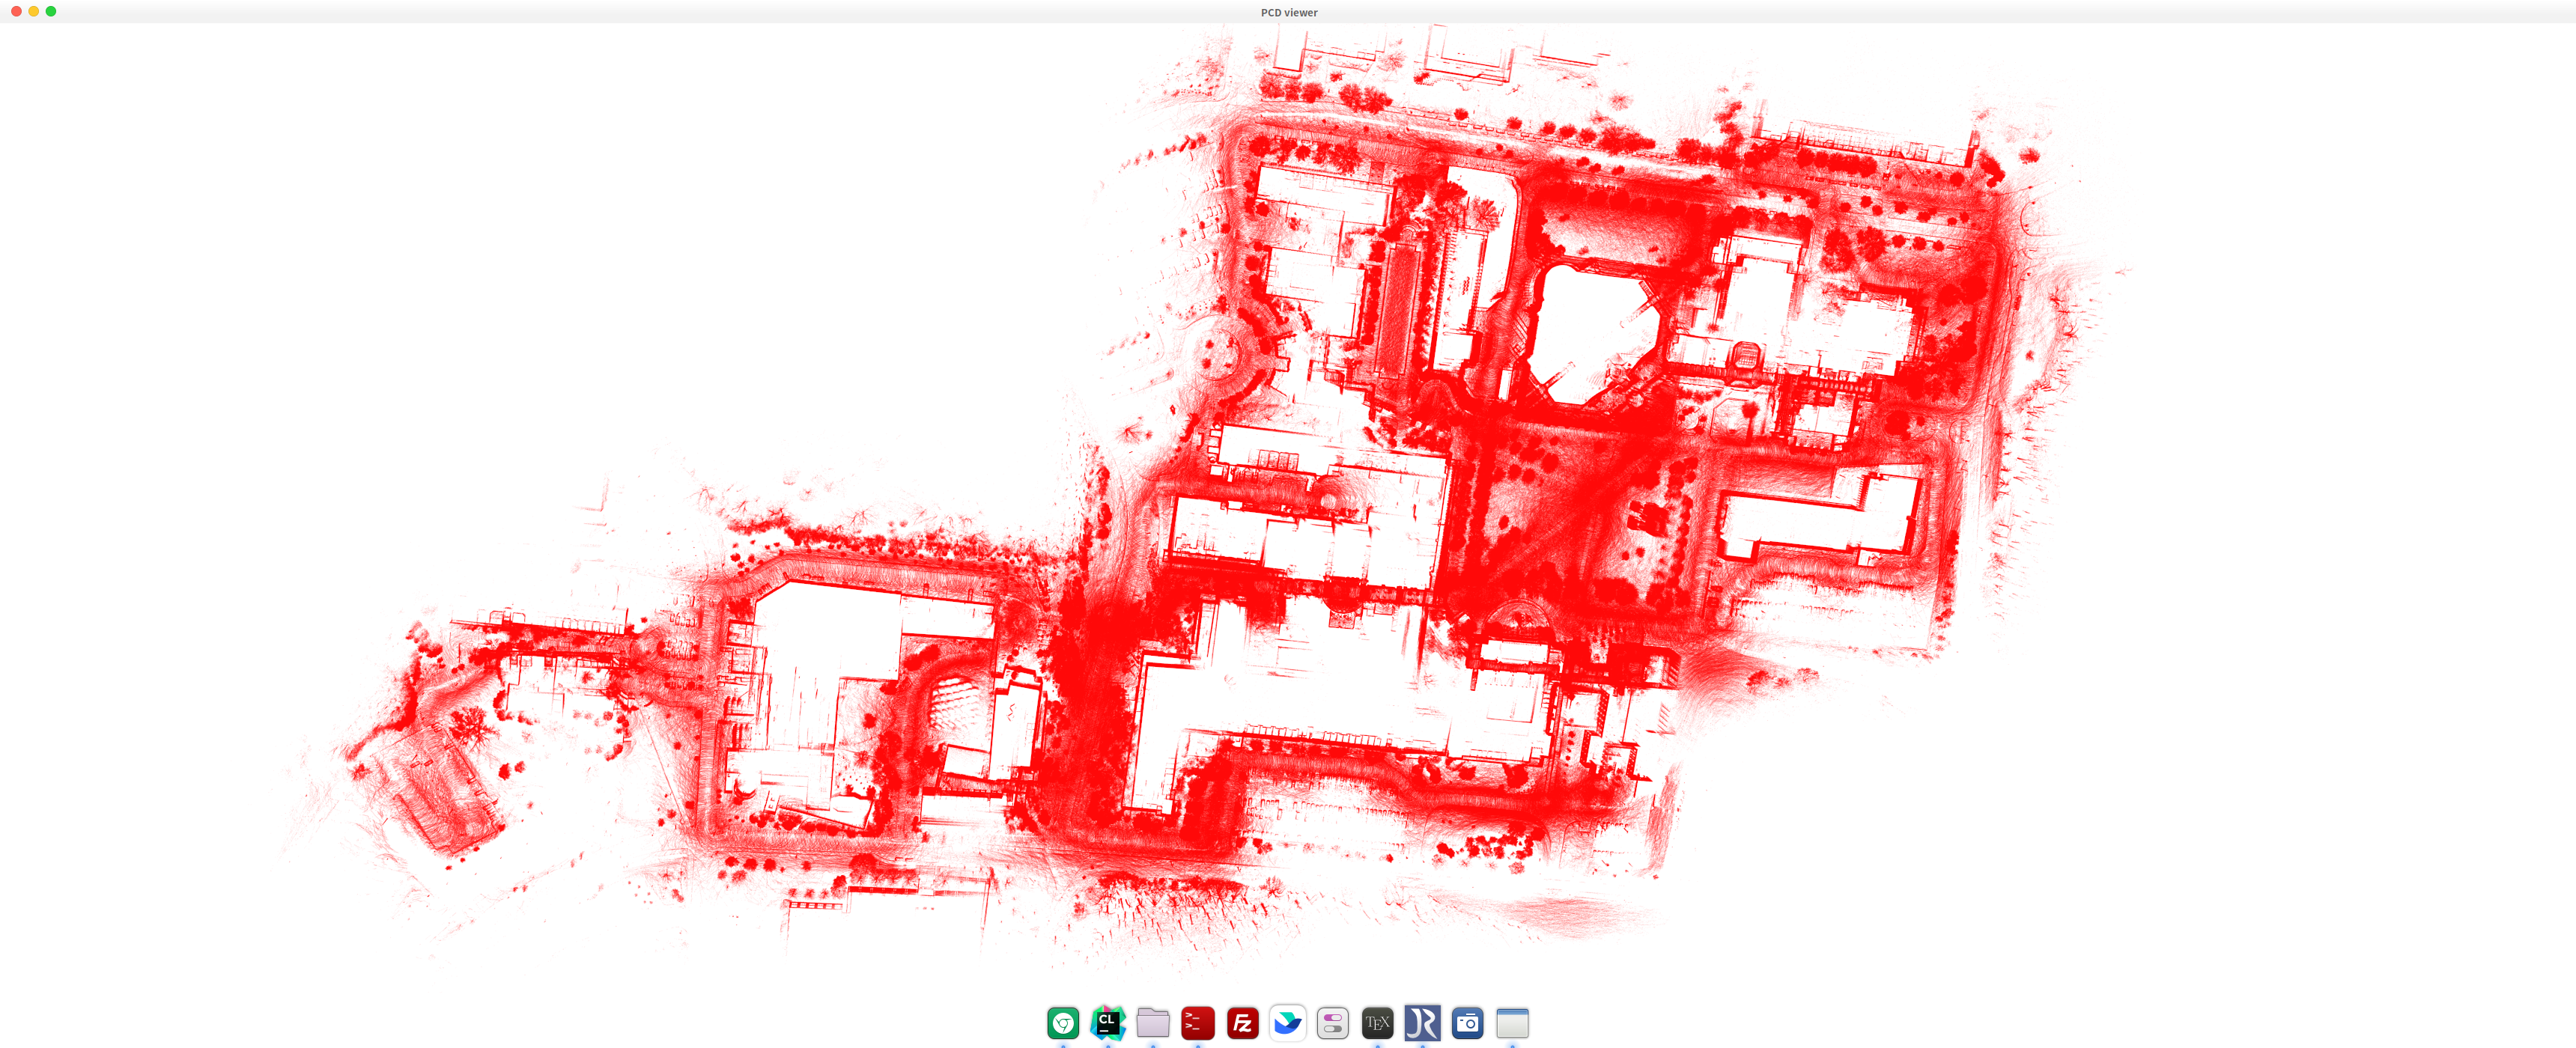
\includegraphics[width=1.0\textwidth]{mapping/nclt-lidar}
	\caption{NCLT dataset visualization using frontend-estimated poses, showing noticeable ghosting in boxed areas.}
	\label{fig:nclt-frontend}
\end{figure}

The subsequent mapping pipeline can start from the frontend results without reprocessing ROS bags. Compared to raw data, keyframe data is significantly smaller due to distance/angle subsampling (55GB raw NCLT data vs 2GB keyframe data). Next we'll perform joint optimization using RTK and LIO poses, followed by loop closure detection to eliminate accumulated errors.

\section{Backend Pose Graph Optimization and Outlier Detection}
First, let's examine the backend pose graph optimization algorithm. We want the final optimized trajectory to incorporate inputs from various sensors, so the backend graph optimization needs to include these factors:
\begin{itemize}
	\item RTK factors. RTK factors provide absolute pose observations. If the dataset includes attitude information, we incorporate it. If only translation is available, we only build translation-related constraints. As discussed in Chapter~\ref{cpt:ins}, when RTK has extrinsic parameters, its translation observations need transformation before correctly affecting vehicle displacement. This is implemented in our code.
	\item LiDAR odometry information. We use the previously introduced LO or LIO as local continuity constraints.
	\item Loop closure factors. If loop closure detection is performed, we load the relevant information and incorporate it into the graph optimization.
\end{itemize}

These three factors constitute our fundamental pose graph optimization problem. We implement their definitions within the g2o framework:

\begin{lstlisting}[language=c++,caption=src/common/g2o\_types.h]
/**
* 3-DOF GNSS constraint
**/
class EdgeGNSSTransOnly : public g2o::BaseUnaryEdge<3, Vec3d, VertexPose> {
	public:
	EIGEN_MAKE_ALIGNED_OPERATOR_NEW;
	EdgeGNSSTransOnly() = default;
	EdgeGNSSTransOnly(VertexPose* v, const Vec3d& obs, const SE3& TBG = SE3()) {
		setVertex(0, v);
		setMeasurement(obs);
		TBG_ = TBG;
	}
	
	void computeError() override {
		VertexPose* v = (VertexPose*)_vertices[0];
		_error = (v->estimate() * TBG_).translation() - _measurement;
	};
	
	void linearizeOplus() override {
		// jacobian 3x6
		VertexPose* v = (VertexPose*)_vertices[0];
		SE3 TWB = v->estimate();
		_jacobianOplusXi.setZero();
		_jacobianOplusXi.block<3, 3>(0, 0) = -TWB.so3().matrix() * SO3::hat(TBG_.translation());
		_jacobianOplusXi.block<3, 3>(0, 3) = Mat3d::Identity();
	}
	
	private:
	SE3 TBG_;
};

/**
* 6-DOF relative motion constraint
* Error order: translation first, then rotation
* Observation: T12
*/
class EdgeRelativeMotion : public g2o::BaseBinaryEdge<6, SE3, VertexPose, VertexPose> {
	public:
	EIGEN_MAKE_ALIGNED_OPERATOR_NEW;
	EdgeRelativeMotion() = default;
	EdgeRelativeMotion(VertexPose* v1, VertexPose* v2, const SE3& obs) {
		setVertex(0, v1);
		setVertex(1, v2);
		setMeasurement(obs);
	}
	
	void computeError() override {
		VertexPose* v1 = (VertexPose*)_vertices[0];
		VertexPose* v2 = (VertexPose*)_vertices[1];
		SE3 T12 = v1->estimate().inverse() * v2->estimate();
		_error = (_measurement.inverse() * v1->estimate().inverse() * v2->estimate()).log();
	};
};
\end{lstlisting}

Here, VertexPose represents the pose vertex, EdgeGNSSTransOnly handles single-antenna GNSS observations (including GNSS extrinsic parameters), while LiDAR and loop closure observations are described by the relative motion constraint EdgeRelativeMotion. Before optimization, we construct these vertices and edges, set appropriate weights and kernel functions, and then place them in the optimizer.

The relevant code for building the optimization problem is:

\begin{lstlisting}[language=c++,caption=src/ch9/optimization.cc]
void Optimization::BuildProblem() {
	using BlockSolverType = g2o::BlockSolverX;
	using LinearSolverType = g2o::LinearSolverEigen<BlockSolverType::PoseMatrixType>;
	auto* solver = new g2o::OptimizationAlgorithmLevenberg(
	g2o::make_unique<BlockSolverType>(g2o::make_unique<LinearSolverType>()));
	
	optimizer_.setAlgorithm(solver);
	
	AddVertices();
	AddRTKEdges();
	AddLidarEdges();
	AddLoopEdges();
}
\end{lstlisting}

We won't detail every function for adding vertices and edges in the book - readers can refer to the corresponding code in the repository. After building the complete problem, we first optimize with robust kernels, then remove the kernels from outliers and optimize again. This helps eliminate the impact of outliers. Additionally, if RTK contains no attitude information throughout, the LiDAR odometry trajectory might differ from the RTK trajectory by a rotation. We perform an ICP on the trajectory to estimate this rotation.

Readers can execute an optimization round by running:

\begin{lstlisting}[language=sh,caption=Terminal command:]
bin/run_optimization --stage=1
\end{lstlisting}

The optimization results are written to keyframes.txt and can be visualized using:

\begin{lstlisting}[language=sh,caption=Terminal command:]
python3 scripts/all_path.py ./data/ch9/keyframes.txt 
\end{lstlisting}

As shown in Fig~\ref{fig:opti1-traj}, after the first optimization round, the RTK trajectory largely coincides with the optimized trajectory, and some failure regions are well identified. However, point clouds may still show ghosting since we haven't performed loop closure detection yet.

\begin{figure}
	\centering
	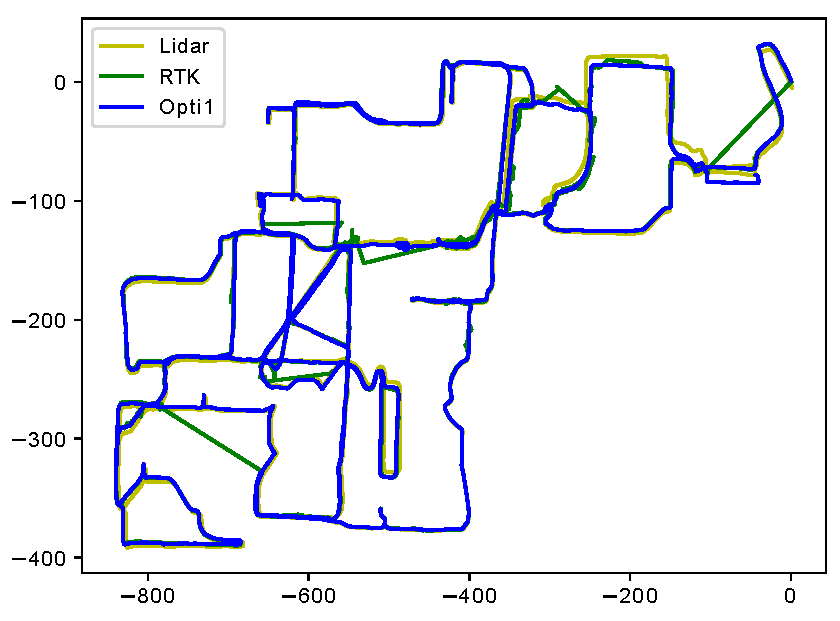
\includegraphics[width=0.6\textwidth]{mapping/opti1_traj}
	\caption{Trajectories after the first optimization round.}
	\label{fig:opti1-traj}
\end{figure}


\section{Loop Closure Detection}
The quality of the point cloud map largely depends on thorough loop closure detection. Without loop closure detection, the shape of the point cloud would primarily rely on the state of the LiDAR odometry. However, LiDAR odometry algorithms only process point clouds from consecutive timestamps, which means that while our map point cloud remains correct under continuous motion, observations from different times and locations are not well-registered. In the loop closure detection step, we aim to design an algorithmic pipeline that enables the program to thoroughly register unaligned regions. Of course, the specific implementation of loop closure detection is flexible—the approach introduced in the book is straightforward and easy to teach. Moreover, since the system operates offline, we can check all relevant regions in one go without waiting for frontend construction results as in real-time operation. During matching, we can also leverage parallel mechanisms to accelerate the loop closure detection process.

We design the loop closure detection steps as follows:
\begin{enumerate}
	\item First, we traverse the keyframes in the first-round optimized trajectory. For each pair of keyframes that are spatially close but temporally distant, we perform a loop closure detection. We refer to such a keyframe pair as a \textbf{checkpoint}. To prevent an excessive number of checkpoints, we set an ID interval, i.e., skipping a fixed number of keyframes between checks. In experiments, this interval is set to 5.
	\item For each keyframe pair, we use a \textbf{scan-to-map} registration method: extracting a subset of the point cloud near the keyframe as a submap, then registering the scan to this submap. This approach mitigates issues arising from insufficient point density or texture in single scans, though it comes with higher computational costs.
	\item Since the computation for each checkpoint is independent, we employ concurrent programming to execute step 2 in parallel, speeding up the process.
	\item The actual registration is performed using NDT (Normal Distributions Transform), and we use the NDT score to determine the validity of the loop closure. Unlike odometry methods, loop closure registration often deals with poor initial pose estimates, so we prefer algorithms less reliant on initial guesses. Thus, we enhance the NDT method with a coarse-to-fine registration process, similar to the multi-resolution 2D registration introduced in Chapter~\ref{cpt:2d-mapping}.
	\item Finally, we record all successful loop closures and read these results during the next optimization call.
\end{enumerate}

The loop closure detection result is described by a loop candidate pair:
\begin{lstlisting}[language=c++,caption=src/ch9/loopclosure.h]
/**
* Loop closure candidate frame
*/
struct LoopCandidate {
	LoopCandidate() {}
	LoopCandidate(IdType id1, IdType id2, SE3 Tij) : idx1_(id1), idx2_(id2), Tij_(Tij) {}
	
	IdType idx1_ = 0;
	IdType idx2_ = 0;
	SE3 Tij_;
	double ndt_score_ = 0.0;
};
\end{lstlisting}

The detection algorithm follows a simple "detect-then-compute" approach:
\begin{lstlisting}[language=c++,caption=src/ch9/loopclosure.cc]
void LoopClosure::Run() {
	DetectLoopCandidates();
	ComputeLoopCandidates();
	
	SaveResults();
}

void LoopClosure::DetectLoopCandidates() {
	KFPtr check_first = nullptr;
	KFPtr check_second = nullptr;
	
	LOG(INFO) << "detecting loop candidates from pose in stage 1";
	
	// Essentially a nested loop
	for (auto iter_first = keyframes_.begin(); iter_first != keyframes_.end(); ++iter_first) {
		auto kf_first = iter_first->second;
		
		if (check_first != nullptr && abs(int(kf_first->id_) - int(check_first->id_)) <= skip_id_) {
			// Keyframe IDs are too close
			continue;
		}
		
		for (auto iter_second = iter_first; iter_second != keyframes_.end(); ++iter_second) {
			auto kf_second = iter_second->second;
			
			if (check_second != nullptr && abs(int(kf_second->id_) - int(check_second->id_)) <= skip_id_) {
				// Keyframe IDs are too close
				continue;
			}
			
			if (abs(int(kf_first->id_) - int(kf_second->id_)) < min_id_interval_) {
				/// If too close on the same trajectory, skip loop closure
				continue;
			}
			
			Vec3d dt = kf_first->opti_pose_1_.translation() - kf_second->opti_pose_1_.translation();
			double t2d = dt.head<2>().norm();  // x-y distance
			double range_th = min_distance_;
			
			if (t2d < range_th) {
				LoopCandidate c(kf_first->id_, kf_second->id_,
				kf_first->opti_pose_1_.inverse() * kf_second->opti_pose_1_);
				loop_candiates_.emplace_back(c);
				check_first = kf_first;
				check_second = kf_second;
			}
		}
	}
	LOG(INFO) << "detected candidates: " << loop_candiates_.size();
}

void LoopClosure::ComputeLoopCandidates() {
	// Execute computation
	std::for_each(std::execution::par_unseq, loop_candiates_.begin(), loop_candiates_.end(),
	[this](LoopCandidate& c) { ComputeForCandidate(c); });
	// Save successful candidates
	std::vector<LoopCandidate> succ_candidates;
	for (const auto& lc : loop_candiates_) {
		if (lc.ndt_score_ > ndt_score_th_) {
			succ_candidates.emplace_back(lc);
		}
	}
	LOG(INFO) << "success: " << succ_candidates.size() << "/" << loop_candiates_.size();
	
	loop_candiates_.swap(succ_candidates);
}
\end{lstlisting}


The actual computation for loop closure is implemented in `ComputeForCandidate`:

\begin{lstlisting}[language=c++,caption=src/ch9/loopclosure.cc]
void LoopClosure::ComputeForCandidate(sad::LoopCandidate& c) {
	LOG(INFO) << "aligning " << c.idx1_ << " with " << c.idx2_;
	const int submap_idx_range = 40;
	KFPtr kf1 = keyframes_.at(c.idx1_), kf2 = keyframes_.at(c.idx2_);
	
	auto build_submap = [this](int given_id, bool build_in_world) -> CloudPtr {
		CloudPtr submap(new PointCloudType);
		for (int idx = -submap_idx_range; idx < submap_idx_range; idx += 4) {
			int id = idx + given_id;
			if (id < 0) {
				continue;
			}
			auto iter = keyframes_.find(id);
			if (iter == keyframes_.end()) {
				continue;
			}
			
			auto kf = iter->second;
			CloudPtr cloud(new PointCloudType);
			pcl::io::loadPCDFile("./data/ch9/" + std::to_string(id) + ".pcd", *cloud);
			RemoveGround(cloud, 0.1);
			
			if (cloud->empty()) {
				continue;
			}
			
			// Transform to world frame
			SE3 Twb = kf->opti_pose_1_;
			
			if (!build_in_world) {
				Twb = keyframes_.at(given_id)->opti_pose_1_.inverse() * Twb;
			}
			
			CloudPtr cloud_trans(new PointCloudType);
			pcl::transformPointCloud(*cloud, *cloud_trans, Twb.matrix());
			
			*submap += *cloud_trans;
		}
		return submap;
	};
	
	auto submap_kf1 = build_submap(kf1->id_, true);
	
	kf2->cloud_.reset(new PointCloudType);
	pcl::io::loadPCDFile("./data/ch9/" + std::to_string(kf2->id_) + ".pcd", *kf2->cloud_);
	auto submap_kf2 = kf2->cloud_;
	
	if (submap_kf1->empty() || submap_kf2->empty()) {
		c.ndt_score_ = 0;
		return;
	}
	
	pcl::NormalDistributionsTransform<PointType, PointType> ndt;
	
	ndt.setResolution(10.0);
	ndt.setTransformationEpsilon(0.05);
	ndt.setStepSize(0.7);
	ndt.setMaximumIterations(40);
	
	Mat4f Tw2 = kf2->opti_pose_1_.matrix().cast<float>();
	
	/// Multi-resolution matching
	CloudPtr output(new PointCloudType);
	std::vector<double> res{10.0, 5.0, 4.0, 3.0};
	for (auto& r : res) {
		ndt.setResolution(r);
		auto rough_map1 = VoxelCloud(submap_kf1, r * 0.1);
		auto rough_map2 = VoxelCloud(submap_kf2, r * 0.1);
		ndt.setInputTarget(rough_map1);
		ndt.setInputSource(rough_map2);
		
		ndt.align(*output, Tw2);
		Tw2 = ndt.getFinalTransformation();
	}
	
	Mat4d T = Tw2.cast<double>();
	Quatd q(T.block<3, 3>(0, 0));
	q.normalize();
	Vec3d t = T.block<3, 1>(0, 3);
	c.Tij_ = kf1->opti_pose_1_.inverse() * SE3(q, t);
	c.ndt_score_ = ndt.getTransformationProbability();
}
\end{lstlisting}

As shown, we perform registration at grid resolutions of 10, 5, 4, and 3 meters respectively, feeding each registration result into the next iteration. The final score is determined using the 3-meter resolution result.

Now please compile and run the loop closure detection program:
\begin{lstlisting}[language=sh,caption=Terminal command:]
bin/run_loopclosure
\end{lstlisting}

The loop closure detection will run for some time, with duration depending on the number of matches. Please wait patiently. After completion, we execute the second round of pose optimization, which will incorporate the loop closure results:
\begin{lstlisting}[language=sh,caption=Terminal command:]
bin/run_optimization --stage=2
\end{lstlisting}

The optimized poses will be saved to `./data/ch9/after.g2o`. We can visualize the pose graph with loop closures using `g2o_viewer`, as shown in Figure~\ref{fig:loop-closure-viewer}. Observe that correct loop closures are detected in most revisited areas.

\begin{figure}
	\centering
	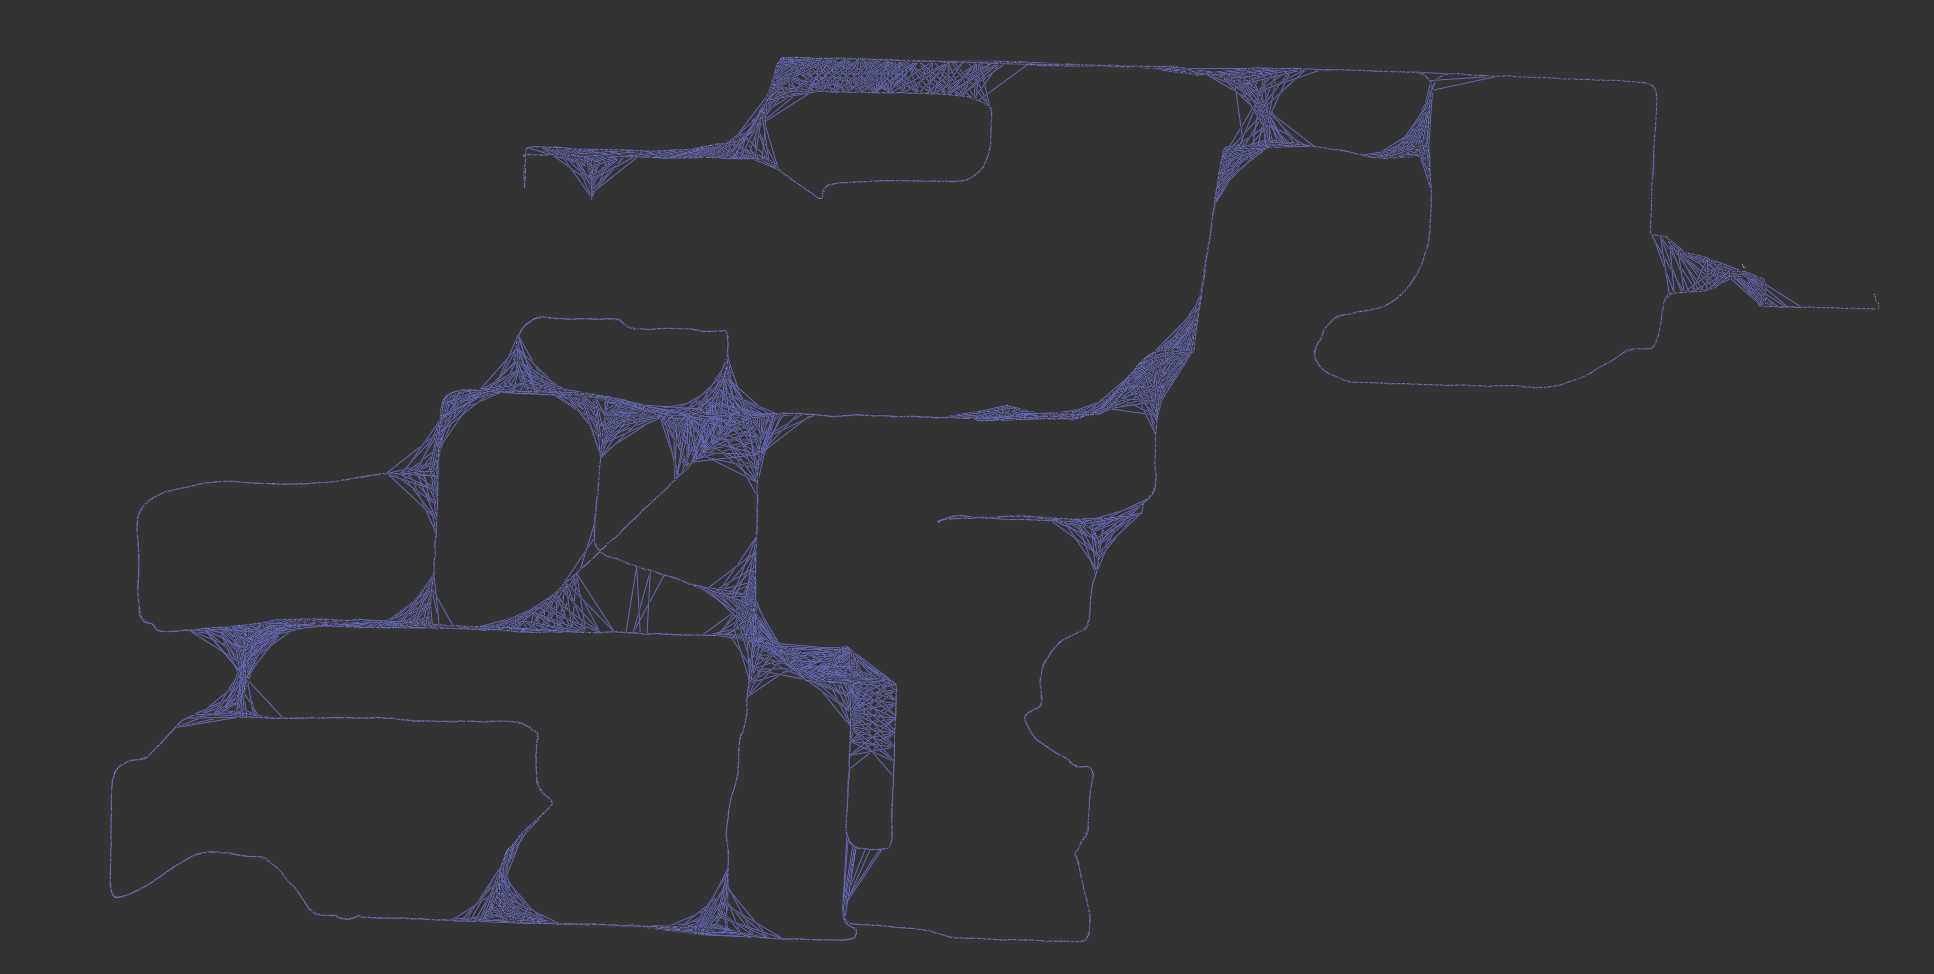
\includegraphics[width=0.8\textwidth]{mapping/viewer.png}
	\caption{Pose graph with loop closures}
	\label{fig:loop-closure-viewer}
\end{figure}

Now export the point cloud after the second optimization round, which should show no significant ghosting artifacts:
\begin{lstlisting}[language=sh,caption=Terminal command:]
/bin/dump_map --pose_source opti2
\end{lstlisting}

\begin{figure}
	\centering
	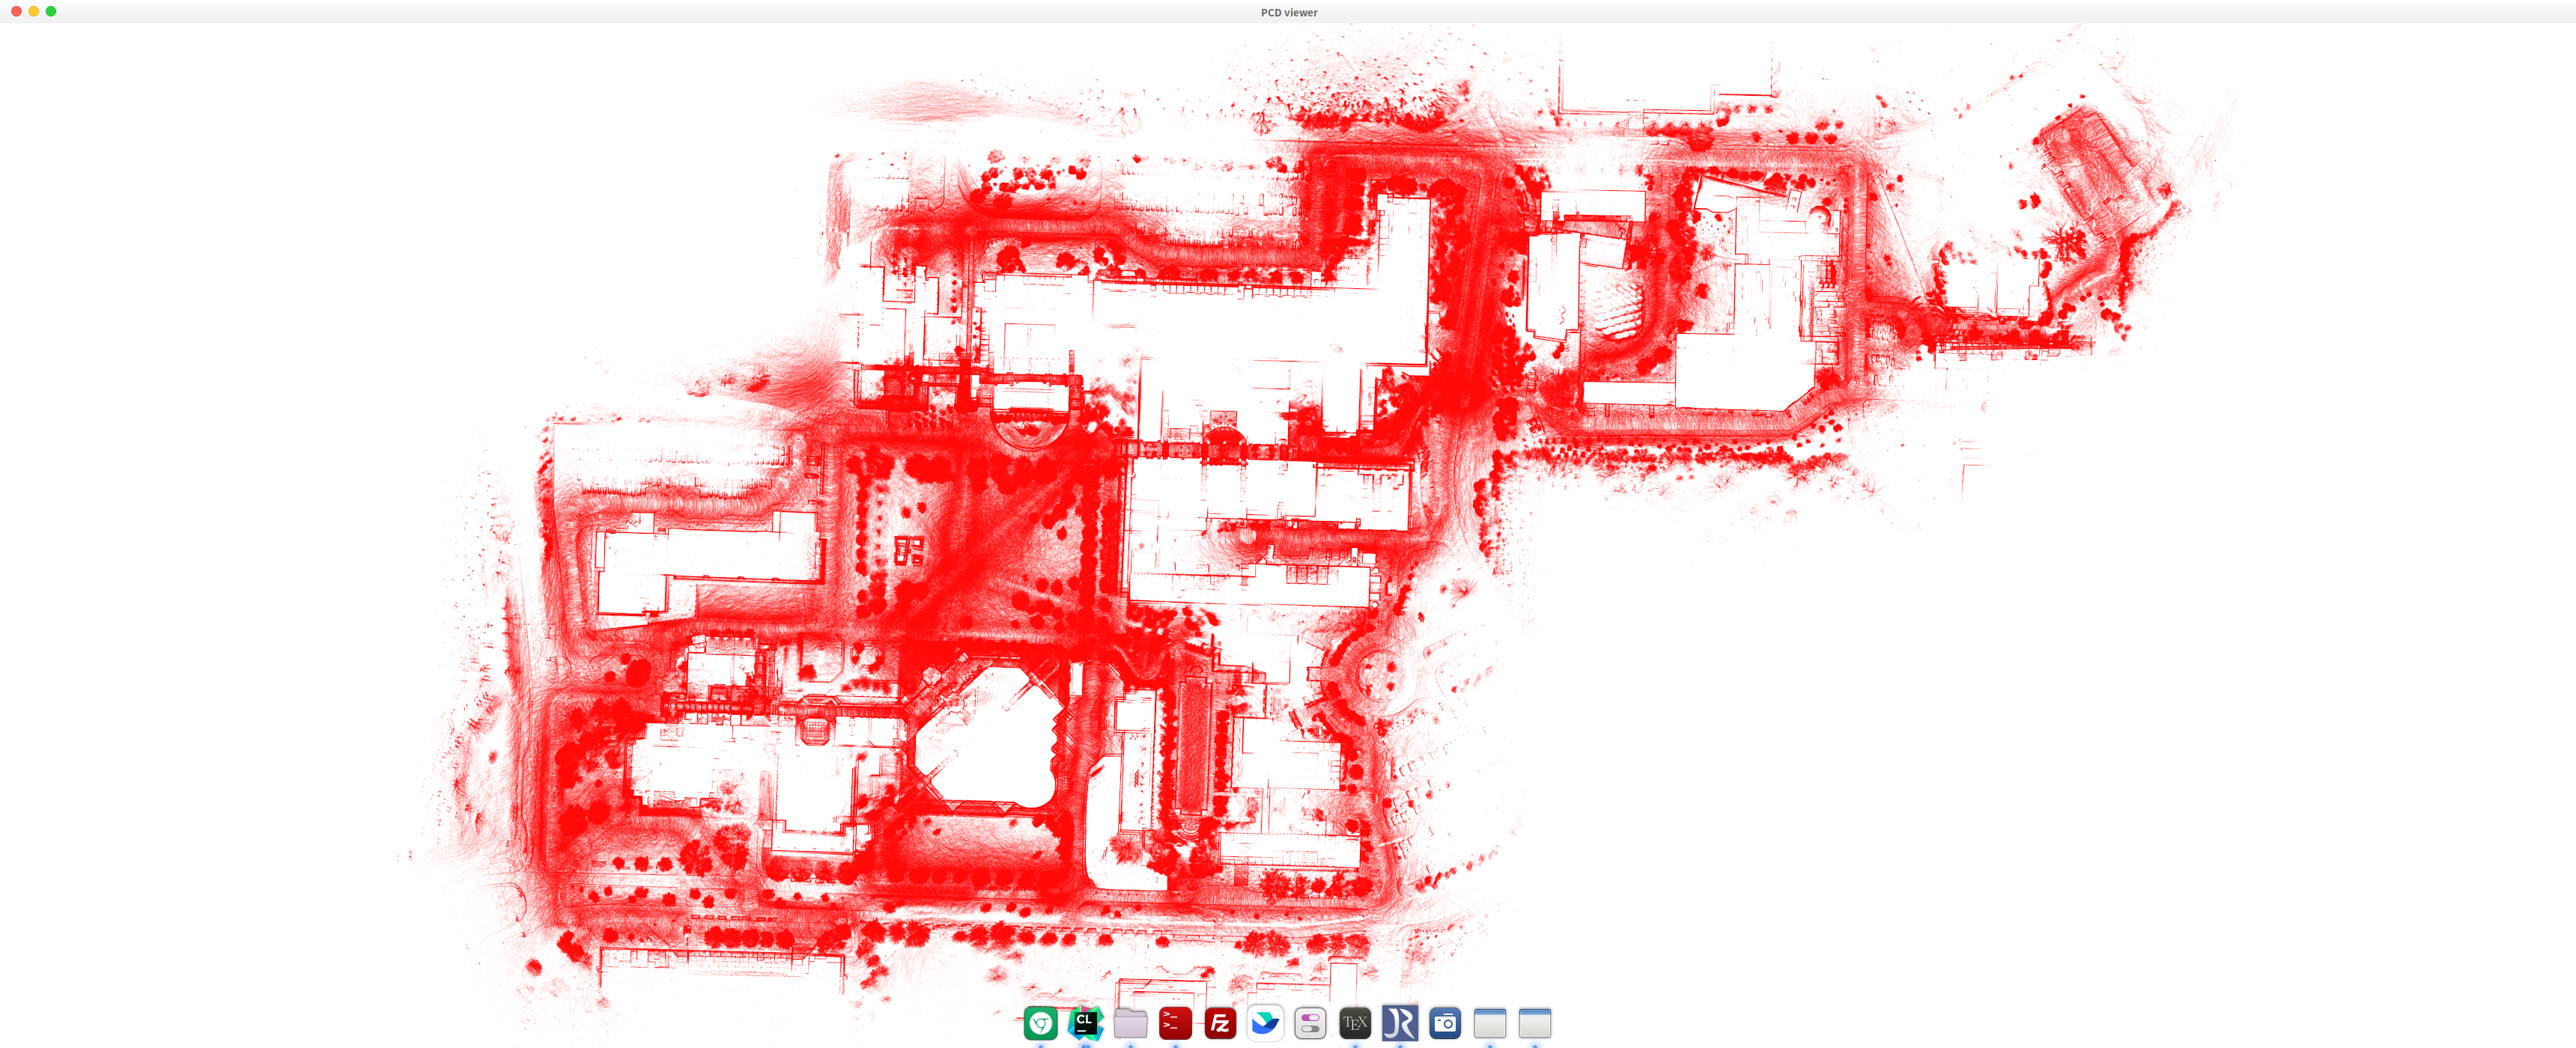
\includegraphics[width=0.8\textwidth]{mapping/map-stage2}
	\caption{Optimized point cloud map after stage 2}
	\label{fig:map-stage2}
\end{figure}

\begin{figure}
	\centering
	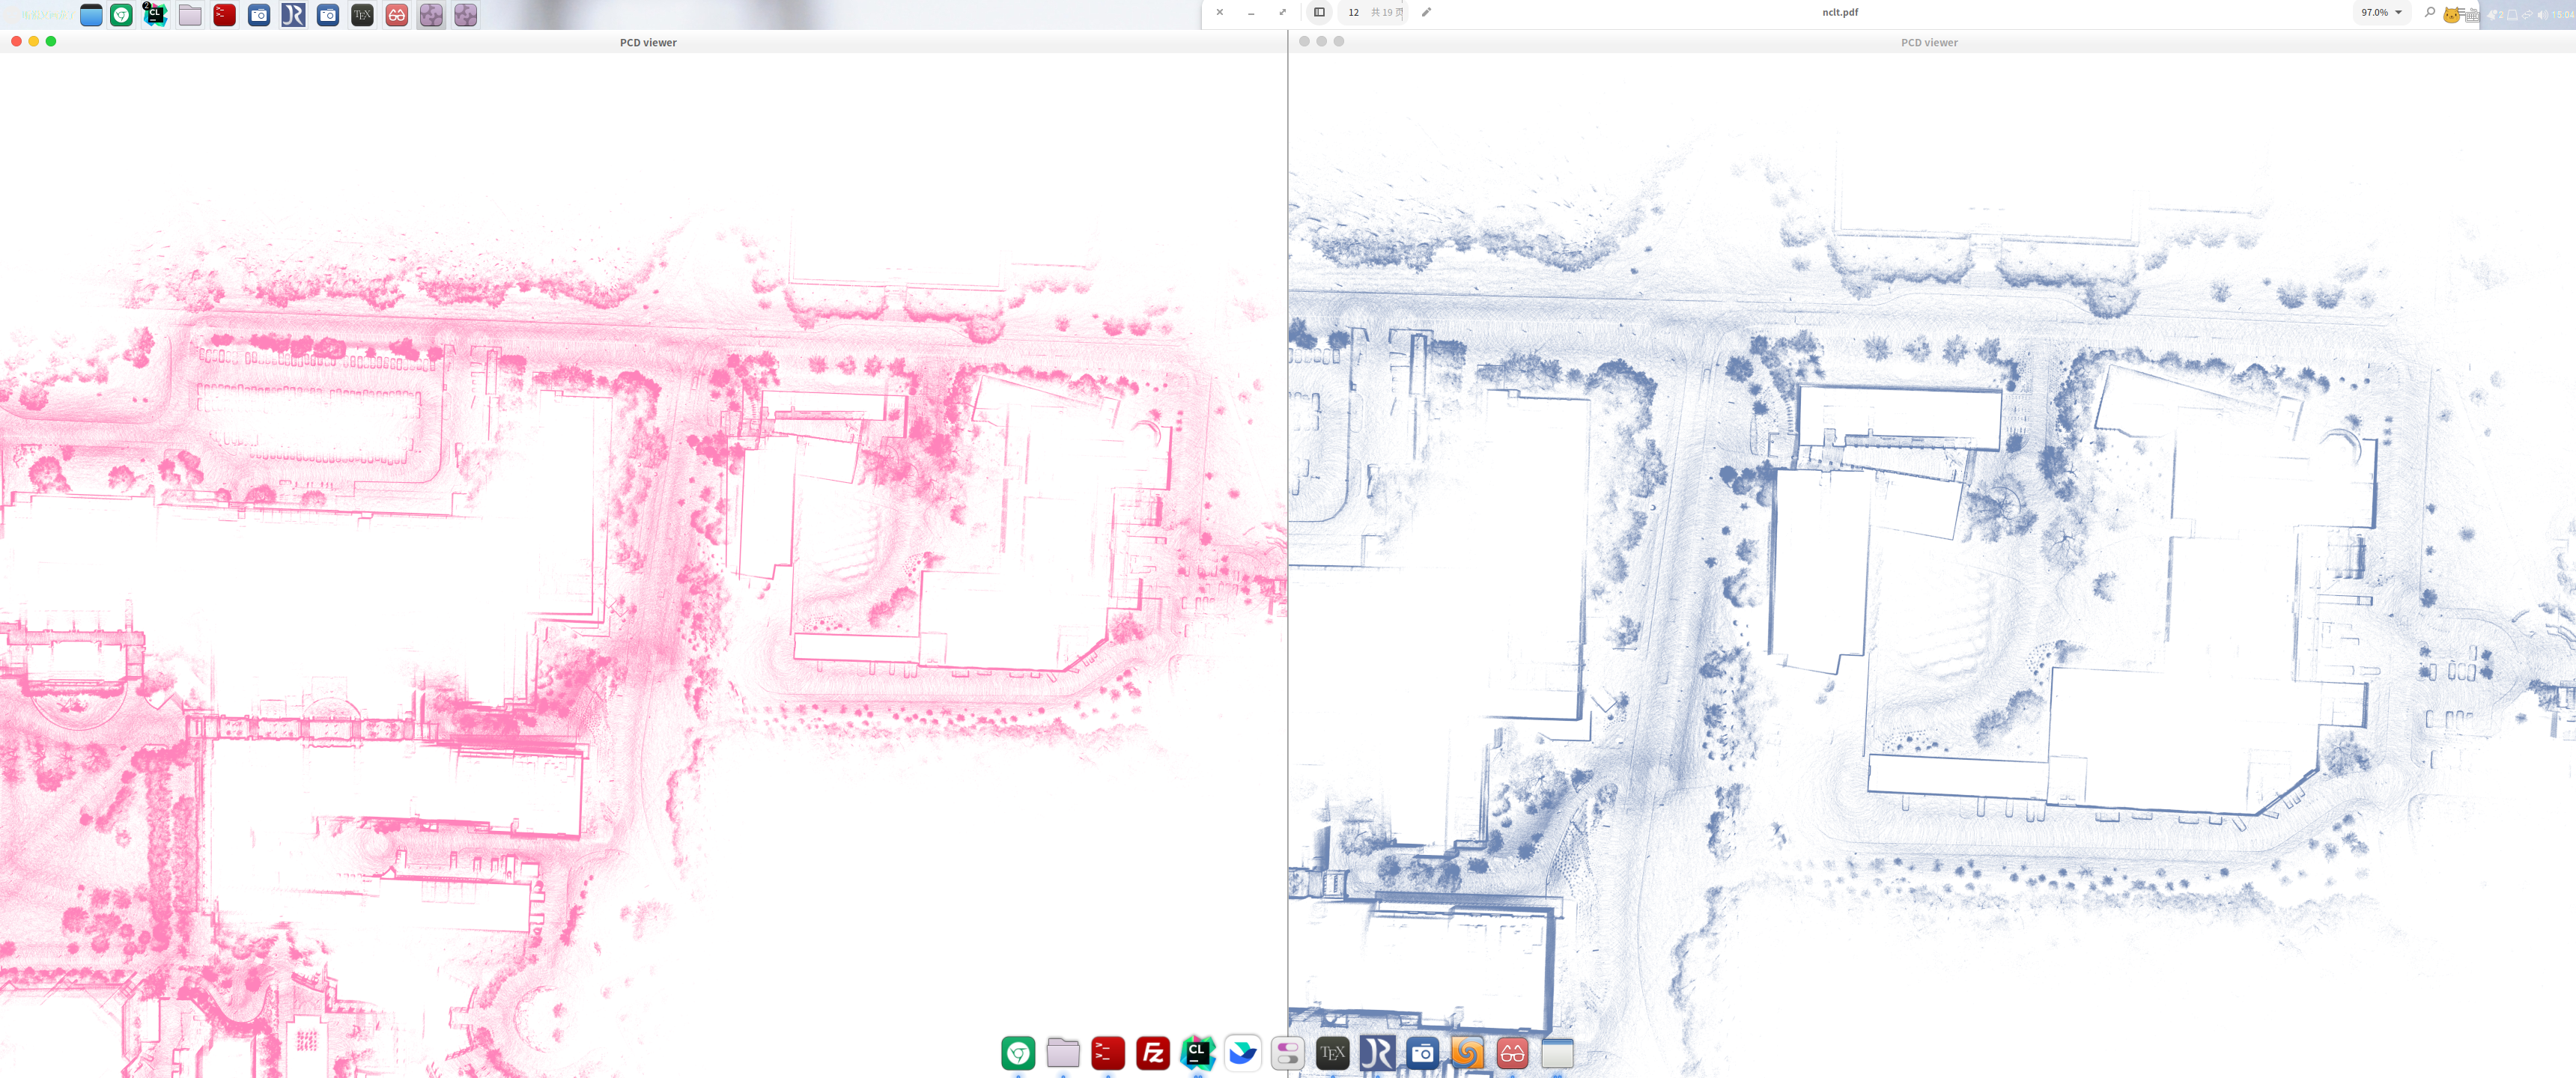
\includegraphics[width=1.0\textwidth]{mapping/compare1}
	\caption{Local comparison between LIO point cloud and optimized point cloud. Left: LIO point cloud, Right: Optimized point cloud}
	\label{fig:map-compare}
\end{figure}

The comparison between pre- and post-optimization point clouds is shown in Figure~\ref{fig:map-compare}. Significant improvement in local details demonstrates that loop closure detection and pose optimization are highly effective components of the pipeline. In practice, loop closure range and registration parameters should be adjusted according to sensor accuracy, but for this dataset, the resulting point cloud is already sufficient for our purposes.

Here is the English translation with LaTeX commands preserved:

\section{Map Export}
Finally, we should export the complete point cloud map. While merging all point clouds into a single map is convenient for visualization, this approach is not ideal for real-time localization systems. In most applications, we want to control the loading scale of real-time point clouds—for example, only loading point clouds within a 200-meter radius around the vehicle and unloading distant regions as needed. This helps manage computational load in real-time systems. Below, we reorganize the point clouds generated in this chapter by splitting them into 100-meter grid blocks and design interfaces for block loading and unloading.

The splitting process essentially calculates the grid ID for each point based on its coordinates and assigns it to the corresponding grid. For more robust implementation, we could incorporate parallelization and batch read/write operations. However, since the dataset used in this chapter is relatively small, the benefits of concurrency are limited, so we demonstrate a single-threaded version here.

\begin{lstlisting}[language=c++,caption=src/ch9/split\_map.cc]
int main(int argc, char** argv) {	
	std::map<IdType, KFPtr> keyframes;
	if (!LoadKeyFrames("./data/ch9/keyframes.txt", keyframes)) {
		LOG(ERROR) << "failed to load keyframes";
		return 0;
	}
	
	std::map<Vec2i, CloudPtr, less_vec<2>> map_data;  // Map data indexed by grid ID
	pcl::VoxelGrid<PointType> voxel_grid_filter;
	float resolution = FLAGS_voxel_size;
	voxel_grid_filter.setLeafSize(resolution, resolution, resolution);
	
	// Logic similar to dump_map: Find/create grid ID for each point
	for (auto& kfp : keyframes) {
		auto kf = kfp.second;
		kf->LoadScan("./data/ch9/");
		
		CloudPtr cloud_trans(new PointCloudType);
		pcl::transformPointCloud(*kf->cloud_, *cloud_trans, kf->opti_pose_2_.matrix());
		
		// Apply voxel filtering
		CloudPtr kf_cloud_voxeled(new PointCloudType);
		voxel_grid_filter.setInputCloud(cloud_trans);
		voxel_grid_filter.filter(*kf_cloud_voxeled);
		
		LOG(INFO) << "building kf " << kf->id_ << " in " << keyframes.size();
		
		// Assign points to grids
		for (const auto& pt : kf_cloud_voxeled->points) {
			int gx = int((pt.x - 50.0) / 100);
			int gy = int((pt.y - 50.0) / 100);
			Vec2i key(gx, gy);
			auto iter = map_data.find(key);
			if (iter == map_data.end()) {
				// Create new point cloud
				CloudPtr cloud(new PointCloudType);
				cloud->points.emplace_back(pt);
				cloud->is_dense = false;
				cloud->height = 1;
				map_data.emplace(key, cloud);
			} else {
				iter->second->points.emplace_back(pt);
			}
		}
	}
	
	// Save point clouds and index file
	LOG(INFO) << "saving maps, grids: " << map_data.size();
	std::system("mkdir -p ./data/ch9/map_data/");
	std::system("rm -rf ./data/ch9/map_data/*");  // Clear directory
	std::ofstream fout("./data/ch9/map_data/map_index.txt");
	for (auto& dp : map_data) {
		fout << dp.first[0] << " " << dp.first[1] << std::endl;
		dp.second->width = dp.second->size();
		VoxelGrid(dp.second, 0.1);
		
		pcl::io::savePCDFileBinaryCompressed(
		"./data/ch9/map_data/" + std::to_string(dp.first[0]) + "_" + std::to_string(dp.first[1]) + ".pcd",
		*dp.second);
	}
	fout.close();
	
	LOG(INFO) << "done.";
	return 0;
}
\end{lstlisting}

After splitting, each map block is exported as a separate PCD file. An index file (map\_index.txt) stores grid locations in text format for quick access. The split point clouds can still be visualized using pcl\_viewer with color-coded blocks, as shown in Figure~\ref{fig:map-grids}. This demonstrates a 100-meter grid splitting scheme, which readers may adapt to larger or smaller block sizes.

\begin{figure}
	\centering
	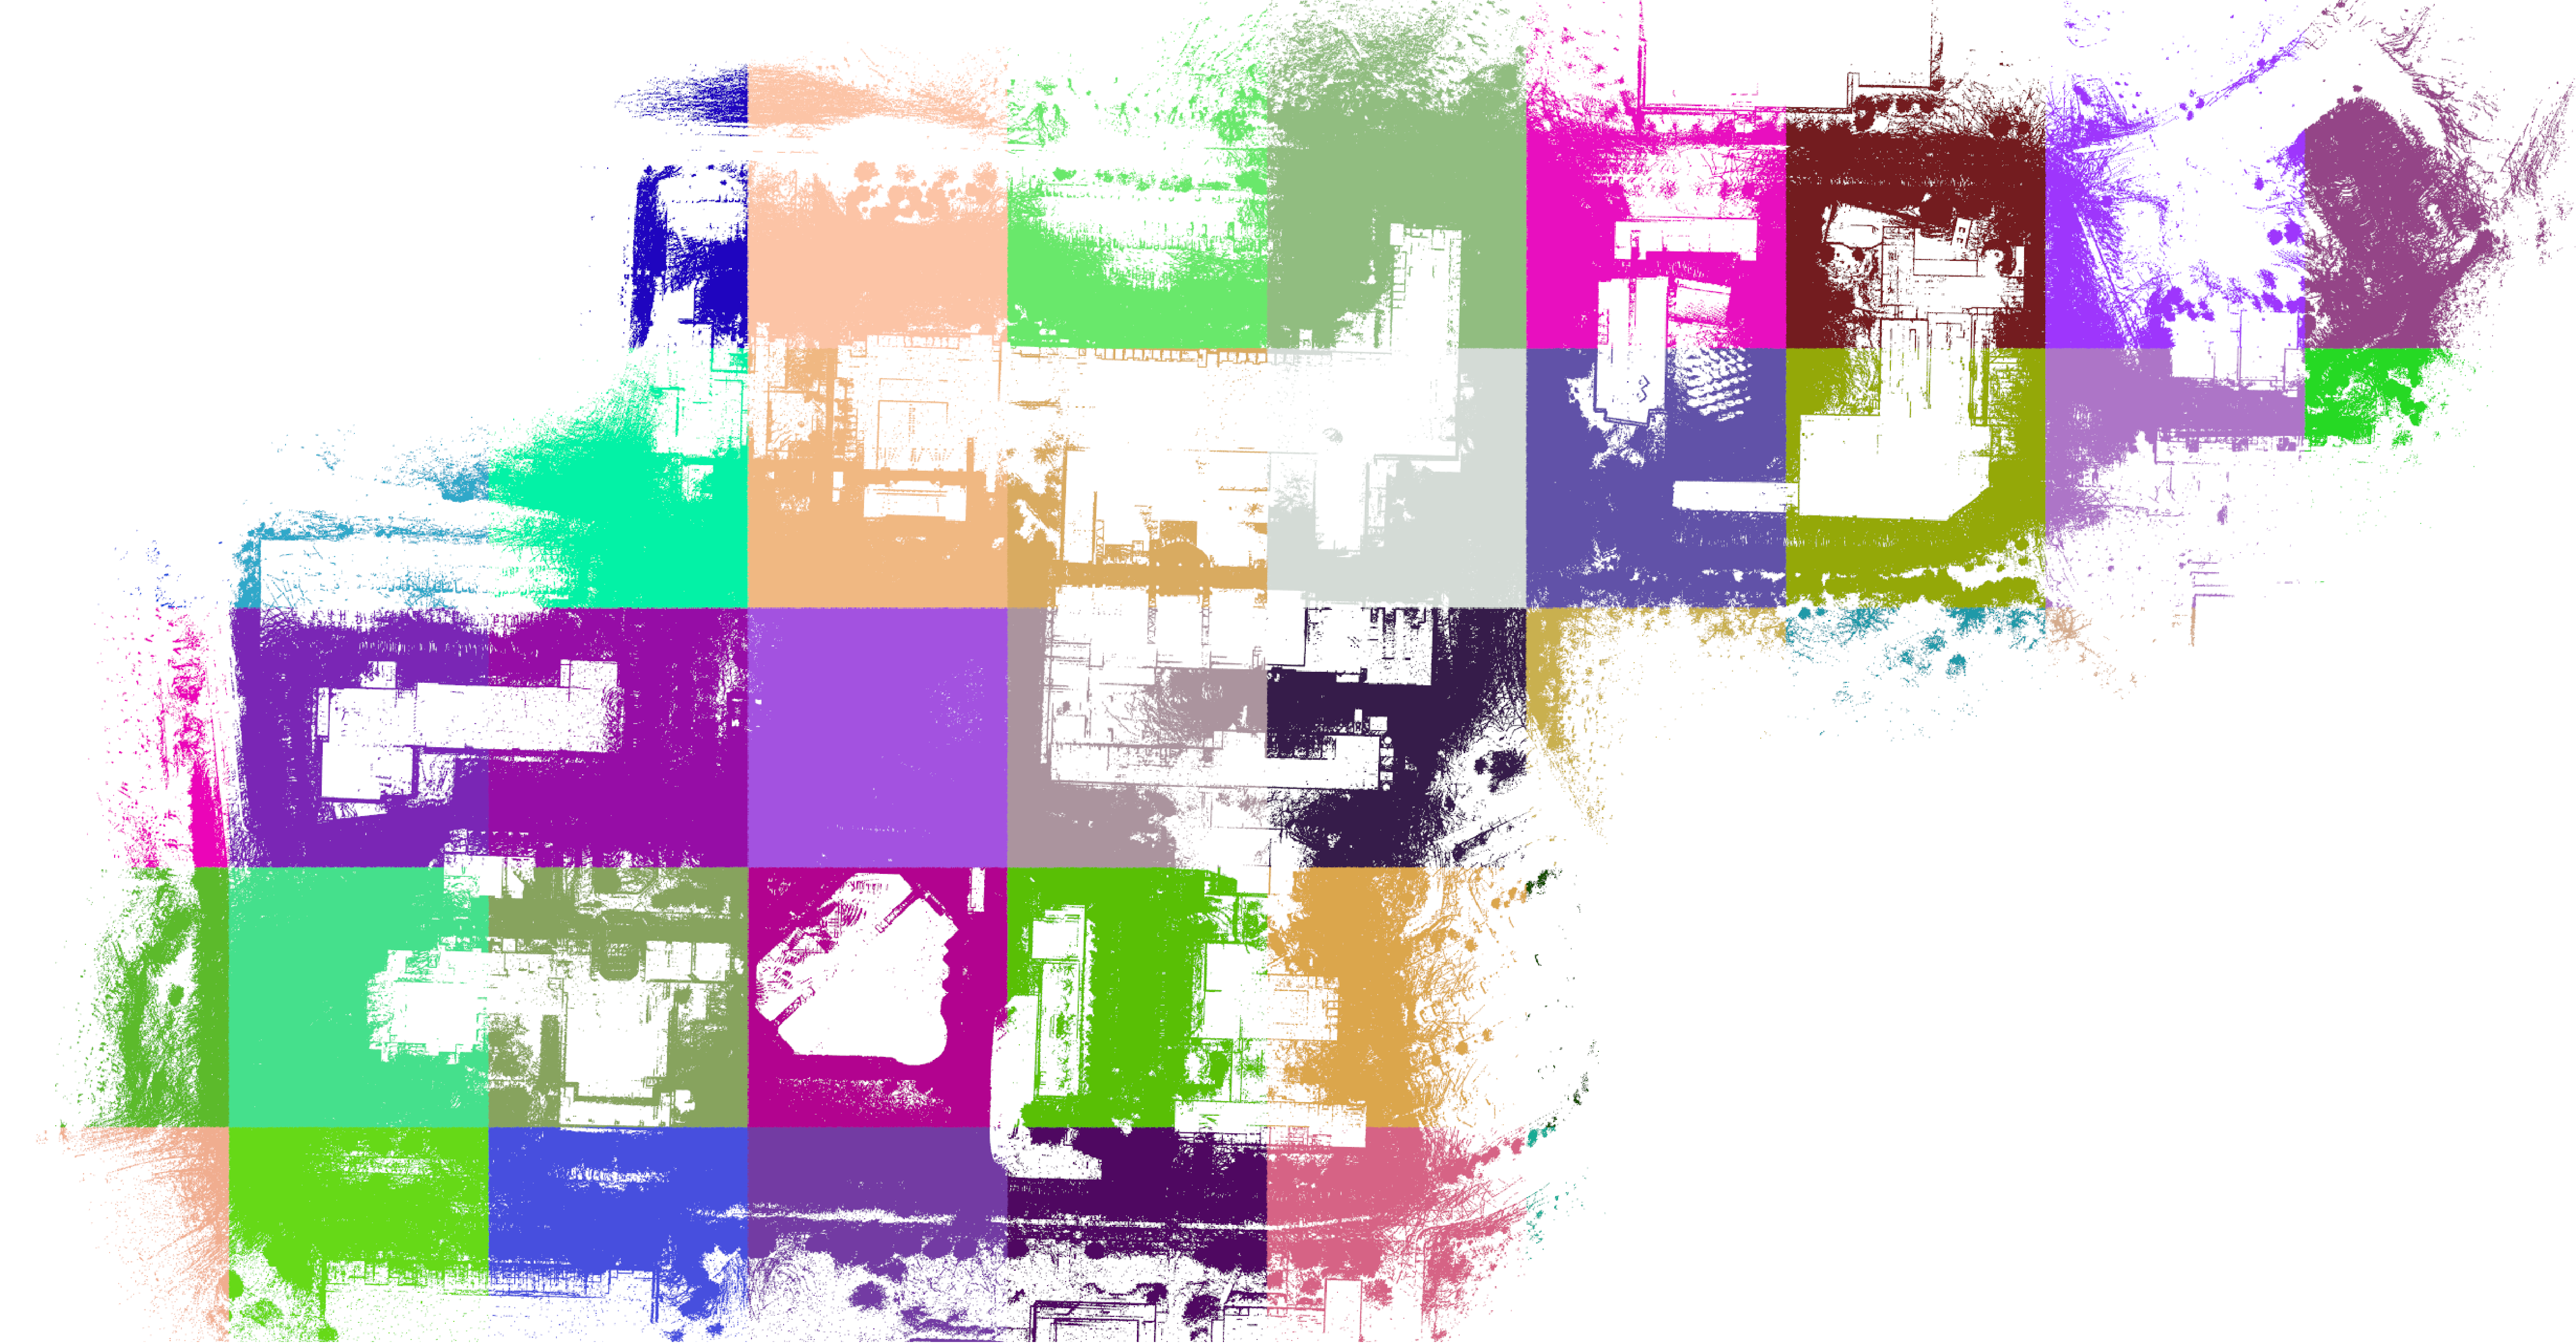
\includegraphics[width=0.8\textwidth]{mapping/map_grids}
	\caption{Split point cloud map}
	\label{fig:map-grids}
\end{figure}

\section{Summary}  
This chapter demonstrated a complete pipeline for point cloud mapping, optimization, and segmentation. The entire mapping process is highly streamlined and automated. By sequentially executing the programs described in this chapter, users can complete a full mapping procedure.  

\begin{lstlisting}[language=c++,caption=src/ch9/run_mapping.cc]  
int main(int argc, char** argv) {  
	google::InitGoogleLogging(argv[0]);  
	FLAGS_stderrthreshold = google::INFO;  
	FLAGS_colorlogtostderr = true;  
	google::ParseCommandLineFlags(&argc, &argv, true);  
	
	LOG(INFO) << "testing frontend";  
	sad::Frontend frontend(FLAGS_config_yaml);  
	if (!frontend.Init()) {  
		LOG(ERROR) << "failed to init frontend.";  
		return -1;  
	}  
	
	frontend.Run();  
	
	sad::Optimization opti(FLAGS_config_yaml);  
	if (!opti.Init(1)) {  
		LOG(ERROR) << "failed to init opti1.";  
		return -1;  
	}  
	opti.Run();  
	
	sad::LoopClosure lc(FLAGS_config_yaml);  
	if (lc.Init() == false) {  
		LOG(ERROR) << "failed to init loop closure.";  
		return -1;  
	}  
	lc.Run();  
	
	sad::Optimization opti2(FLAGS_config_yaml);  
	if (!opti2.Init(2)) {  
		LOG(ERROR) << "failed to init opti1.";  
		return -1;  
	}  
	opti2.Run();  
	
	LOG(INFO) << "done.";  
	return 0;  
}  
\end{lstlisting}  

By simply specifying an NCLT dataset in the configuration file, the program automatically constructs a complete point cloud map with loop closure corrections. Readers are encouraged to test this pipeline on other NCLT datasets and compare their performance. These maps facilitate \textbf{high-precision LiDAR localization}, enabling vehicles and robots to achieve accurate pose estimation without RTK. In the next chapter, we will utilize the point cloud maps built here for real-time high-precision localization.  

\section*{Exercises}  
\begin{enumerate}  
	\item Modify the frontend of this chapter's mapping pipeline to use LOAM or its variants, and compare their performance with the LIO frontend employed in this book.  
	\item Replace the loop closure detection backend with Scan Context or other registration methods to improve its stability.  
	\item Adapt the NDT registration used for loop closure to the NDT implementation from Chapter 7. Design your own metric for match scoring.  
\end{enumerate}


